% Options for packages loaded elsewhere
\PassOptionsToPackage{unicode}{hyperref}
\PassOptionsToPackage{hyphens}{url}
%
\documentclass[
]{article}
\usepackage{lmodern}
\usepackage{amssymb,amsmath}
\usepackage{ifxetex,ifluatex}
\ifnum 0\ifxetex 1\fi\ifluatex 1\fi=0 % if pdftex
  \usepackage[T1]{fontenc}
  \usepackage[utf8]{inputenc}
  \usepackage{textcomp} % provide euro and other symbols
\else % if luatex or xetex
  \usepackage{unicode-math}
  \defaultfontfeatures{Scale=MatchLowercase}
  \defaultfontfeatures[\rmfamily]{Ligatures=TeX,Scale=1}
\fi
% Use upquote if available, for straight quotes in verbatim environments
\IfFileExists{upquote.sty}{\usepackage{upquote}}{}
\IfFileExists{microtype.sty}{% use microtype if available
  \usepackage[]{microtype}
  \UseMicrotypeSet[protrusion]{basicmath} % disable protrusion for tt fonts
}{}
\makeatletter
\@ifundefined{KOMAClassName}{% if non-KOMA class
  \IfFileExists{parskip.sty}{%
    \usepackage{parskip}
  }{% else
    \setlength{\parindent}{0pt}
    \setlength{\parskip}{6pt plus 2pt minus 1pt}}
}{% if KOMA class
  \KOMAoptions{parskip=half}}
\makeatother
\usepackage{xcolor}
\IfFileExists{xurl.sty}{\usepackage{xurl}}{} % add URL line breaks if available
\IfFileExists{bookmark.sty}{\usepackage{bookmark}}{\usepackage{hyperref}}
\hypersetup{
  pdftitle={Anny\_Tarea-02.R},
  pdfauthor={Usuario},
  hidelinks,
  pdfcreator={LaTeX via pandoc}}
\urlstyle{same} % disable monospaced font for URLs
\usepackage[margin=1in]{geometry}
\usepackage{color}
\usepackage{fancyvrb}
\newcommand{\VerbBar}{|}
\newcommand{\VERB}{\Verb[commandchars=\\\{\}]}
\DefineVerbatimEnvironment{Highlighting}{Verbatim}{commandchars=\\\{\}}
% Add ',fontsize=\small' for more characters per line
\usepackage{framed}
\definecolor{shadecolor}{RGB}{248,248,248}
\newenvironment{Shaded}{\begin{snugshade}}{\end{snugshade}}
\newcommand{\AlertTok}[1]{\textcolor[rgb]{0.94,0.16,0.16}{#1}}
\newcommand{\AnnotationTok}[1]{\textcolor[rgb]{0.56,0.35,0.01}{\textbf{\textit{#1}}}}
\newcommand{\AttributeTok}[1]{\textcolor[rgb]{0.77,0.63,0.00}{#1}}
\newcommand{\BaseNTok}[1]{\textcolor[rgb]{0.00,0.00,0.81}{#1}}
\newcommand{\BuiltInTok}[1]{#1}
\newcommand{\CharTok}[1]{\textcolor[rgb]{0.31,0.60,0.02}{#1}}
\newcommand{\CommentTok}[1]{\textcolor[rgb]{0.56,0.35,0.01}{\textit{#1}}}
\newcommand{\CommentVarTok}[1]{\textcolor[rgb]{0.56,0.35,0.01}{\textbf{\textit{#1}}}}
\newcommand{\ConstantTok}[1]{\textcolor[rgb]{0.00,0.00,0.00}{#1}}
\newcommand{\ControlFlowTok}[1]{\textcolor[rgb]{0.13,0.29,0.53}{\textbf{#1}}}
\newcommand{\DataTypeTok}[1]{\textcolor[rgb]{0.13,0.29,0.53}{#1}}
\newcommand{\DecValTok}[1]{\textcolor[rgb]{0.00,0.00,0.81}{#1}}
\newcommand{\DocumentationTok}[1]{\textcolor[rgb]{0.56,0.35,0.01}{\textbf{\textit{#1}}}}
\newcommand{\ErrorTok}[1]{\textcolor[rgb]{0.64,0.00,0.00}{\textbf{#1}}}
\newcommand{\ExtensionTok}[1]{#1}
\newcommand{\FloatTok}[1]{\textcolor[rgb]{0.00,0.00,0.81}{#1}}
\newcommand{\FunctionTok}[1]{\textcolor[rgb]{0.00,0.00,0.00}{#1}}
\newcommand{\ImportTok}[1]{#1}
\newcommand{\InformationTok}[1]{\textcolor[rgb]{0.56,0.35,0.01}{\textbf{\textit{#1}}}}
\newcommand{\KeywordTok}[1]{\textcolor[rgb]{0.13,0.29,0.53}{\textbf{#1}}}
\newcommand{\NormalTok}[1]{#1}
\newcommand{\OperatorTok}[1]{\textcolor[rgb]{0.81,0.36,0.00}{\textbf{#1}}}
\newcommand{\OtherTok}[1]{\textcolor[rgb]{0.56,0.35,0.01}{#1}}
\newcommand{\PreprocessorTok}[1]{\textcolor[rgb]{0.56,0.35,0.01}{\textit{#1}}}
\newcommand{\RegionMarkerTok}[1]{#1}
\newcommand{\SpecialCharTok}[1]{\textcolor[rgb]{0.00,0.00,0.00}{#1}}
\newcommand{\SpecialStringTok}[1]{\textcolor[rgb]{0.31,0.60,0.02}{#1}}
\newcommand{\StringTok}[1]{\textcolor[rgb]{0.31,0.60,0.02}{#1}}
\newcommand{\VariableTok}[1]{\textcolor[rgb]{0.00,0.00,0.00}{#1}}
\newcommand{\VerbatimStringTok}[1]{\textcolor[rgb]{0.31,0.60,0.02}{#1}}
\newcommand{\WarningTok}[1]{\textcolor[rgb]{0.56,0.35,0.01}{\textbf{\textit{#1}}}}
\usepackage{graphicx,grffile}
\makeatletter
\def\maxwidth{\ifdim\Gin@nat@width>\linewidth\linewidth\else\Gin@nat@width\fi}
\def\maxheight{\ifdim\Gin@nat@height>\textheight\textheight\else\Gin@nat@height\fi}
\makeatother
% Scale images if necessary, so that they will not overflow the page
% margins by default, and it is still possible to overwrite the defaults
% using explicit options in \includegraphics[width, height, ...]{}
\setkeys{Gin}{width=\maxwidth,height=\maxheight,keepaspectratio}
% Set default figure placement to htbp
\makeatletter
\def\fps@figure{htbp}
\makeatother
\setlength{\emergencystretch}{3em} % prevent overfull lines
\providecommand{\tightlist}{%
  \setlength{\itemsep}{0pt}\setlength{\parskip}{0pt}}
\setcounter{secnumdepth}{-\maxdimen} % remove section numbering

\title{Anny\_Tarea-02.R}
\author{Usuario}
\date{2020-02-25}

\begin{document}
\maketitle

\begin{Shaded}
\begin{Highlighting}[]
\CommentTok{# Ejercicio 1}

\KeywordTok{library}\NormalTok{(plyr) }
\NormalTok{accidentes <-}\StringTok{ }\KeywordTok{c}\NormalTok{(}\DecValTok{0}\NormalTok{,}\DecValTok{1}\NormalTok{,}\DecValTok{0}\NormalTok{,}\DecValTok{2}\NormalTok{,}\DecValTok{2}\NormalTok{,}\DecValTok{1}\NormalTok{,}\DecValTok{4}\NormalTok{,}\DecValTok{3}\NormalTok{,}\DecValTok{0}\NormalTok{,}\DecValTok{1}\NormalTok{,}\DecValTok{5}\NormalTok{,}\DecValTok{1}\NormalTok{,}\DecValTok{2}\NormalTok{,}\DecValTok{3}\NormalTok{,}\DecValTok{4}\NormalTok{,}\DecValTok{0}\NormalTok{,}\DecValTok{1}\NormalTok{,}\DecValTok{1}\NormalTok{,}\DecValTok{3}\NormalTok{,}\DecValTok{4}\NormalTok{) }
\NormalTok{acc <-}\StringTok{ }\KeywordTok{count}\NormalTok{(accidentes) }
\NormalTok{acc }
\end{Highlighting}
\end{Shaded}

\begin{verbatim}
##   x freq
## 1 0    4
## 2 1    6
## 3 2    3
## 4 3    3
## 5 4    3
## 6 5    1
\end{verbatim}

\begin{Shaded}
\begin{Highlighting}[]
\NormalTok{acc}\OperatorTok{$}\NormalTok{rf <-}\StringTok{ }\NormalTok{acc}\OperatorTok{$}\NormalTok{freq}\OperatorTok{/}\KeywordTok{sum}\NormalTok{(acc}\OperatorTok{$}\NormalTok{freq)}\OperatorTok{*}\DecValTok{100} 
\NormalTok{acc }
\end{Highlighting}
\end{Shaded}

\begin{verbatim}
##   x freq rf
## 1 0    4 20
## 2 1    6 30
## 3 2    3 15
## 4 3    3 15
## 5 4    3 15
## 6 5    1  5
\end{verbatim}

\begin{Shaded}
\begin{Highlighting}[]
\KeywordTok{barplot}\NormalTok{(acc}\OperatorTok{$}\NormalTok{rf, }\DataTypeTok{names.arg =}\NormalTok{ acc}\OperatorTok{$}\NormalTok{x, }\DataTypeTok{col=}\StringTok{"red"}\NormalTok{)}
\end{Highlighting}
\end{Shaded}

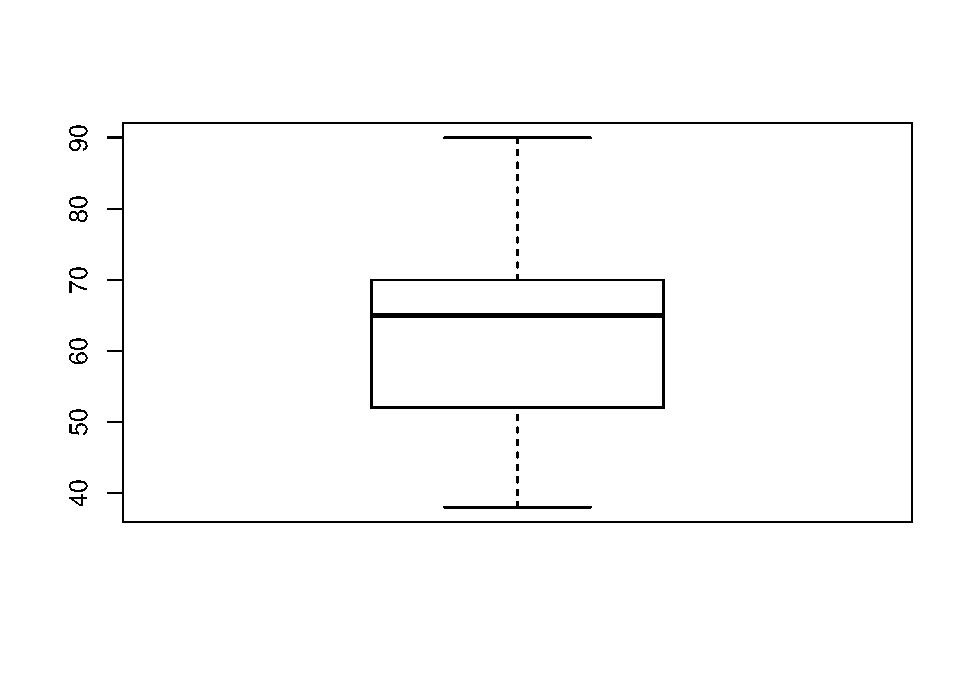
\includegraphics{Anny_Tarea-02_files/figure-latex/unnamed-chunk-1-1.pdf}

\begin{Shaded}
\begin{Highlighting}[]
\CommentTok{# Ejercicio 2}
\NormalTok{especies <-}\StringTok{ }\KeywordTok{c}\NormalTok{(}\StringTok{"F"}\NormalTok{, }\StringTok{"H"}\NormalTok{, }\StringTok{"F"}\NormalTok{, }\StringTok{"C"}\NormalTok{, }\StringTok{"F"}\NormalTok{, }\StringTok{"A"}\NormalTok{, }\StringTok{"H"}\NormalTok{, }\StringTok{"F"}
\NormalTok{              , }\StringTok{"H"}\NormalTok{, }\StringTok{"C"}\NormalTok{, }\StringTok{"A"}\NormalTok{, }\StringTok{"C"}\NormalTok{,}\StringTok{"F"}\NormalTok{, }\StringTok{"H"}\NormalTok{, }\StringTok{"H"}\NormalTok{, }\StringTok{"H"}\NormalTok{,}
              \StringTok{"F"}\NormalTok{, }\StringTok{"H"}\NormalTok{, }\StringTok{"A"}\NormalTok{, }\StringTok{"C"}\NormalTok{, }\StringTok{"F"}\NormalTok{, }\StringTok{"H"}\NormalTok{, }\StringTok{"H"}\NormalTok{, }\StringTok{"F"}\NormalTok{) }

\NormalTok{.sp <-}\StringTok{ }\KeywordTok{count}\NormalTok{(especies) }
\NormalTok{.sp}\OperatorTok{$}\NormalTok{rf <-}\StringTok{ }\NormalTok{.sp}\OperatorTok{$}\NormalTok{freq}\OperatorTok{/}\KeywordTok{sum}\NormalTok{(.sp}\OperatorTok{$}\NormalTok{freq)}\OperatorTok{*}\DecValTok{100} 
\NormalTok{.sp}
\end{Highlighting}
\end{Shaded}

\begin{verbatim}
##   x freq       rf
## 1 A    3 12.50000
## 2 C    4 16.66667
## 3 F    8 33.33333
## 4 H    9 37.50000
\end{verbatim}

\begin{Shaded}
\begin{Highlighting}[]
\KeywordTok{barplot}\NormalTok{(.sp}\OperatorTok{$}\NormalTok{freq, }\DataTypeTok{names.arg =}\NormalTok{ .sp}\OperatorTok{$}\NormalTok{x, }\DataTypeTok{col =} \StringTok{"yellow"}\NormalTok{, }
        \DataTypeTok{ylab =} \StringTok{"Frecuencia"}\NormalTok{, }
        \DataTypeTok{xlab =} \StringTok{"Especies"}\NormalTok{)}
\end{Highlighting}
\end{Shaded}

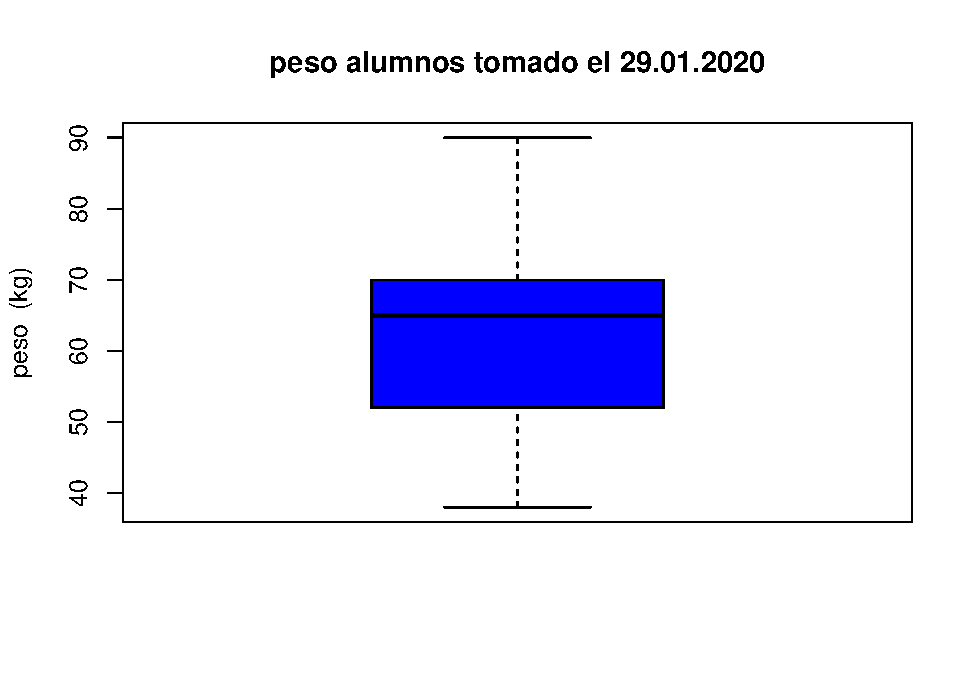
\includegraphics{Anny_Tarea-02_files/figure-latex/unnamed-chunk-1-2.pdf}

\begin{Shaded}
\begin{Highlighting}[]
\CommentTok{# Ejercicio 3}
\KeywordTok{library}\NormalTok{(repmis) }
\NormalTok{conjunto <-}\StringTok{ }\KeywordTok{source_data}\NormalTok{(}\StringTok{"https://www.dropbox.com/s/hmsf07bbayxv6m3/cuadro1.csv?dl=1"}\NormalTok{)}
\end{Highlighting}
\end{Shaded}

\begin{verbatim}
## Downloading data from: https://www.dropbox.com/s/hmsf07bbayxv6m3/cuadro1.csv?dl=1
\end{verbatim}

\begin{verbatim}
## SHA-1 hash of the downloaded data file is:
## 2bdde4663f51aa4198b04a248715d0d93498e7ba
\end{verbatim}

\begin{Shaded}
\begin{Highlighting}[]
\NormalTok{.vc <-}\StringTok{ }\KeywordTok{table}\NormalTok{(conjunto}\OperatorTok{$}\NormalTok{Vecinos, conjunto}\OperatorTok{$}\NormalTok{Especie) }
\NormalTok{.vc1 <-}\StringTok{ }\KeywordTok{addmargins}\NormalTok{(}\KeywordTok{as.table}\NormalTok{(.vc))}
\NormalTok{.vc1 }
\end{Highlighting}
\end{Shaded}

\begin{verbatim}
##      
##        C  F  H Sum
##   0    1  0  2   3
##   1    1  2  1   4
##   2    3  2  1   6
##   3    5  3  5  13
##   4    5  5  3  13
##   5    5  1  0   6
##   6    2  1  2   5
##   Sum 22 14 14  50
\end{verbatim}

\begin{Shaded}
\begin{Highlighting}[]
\CommentTok{# Ejercicio 4}
\NormalTok{.h <-}\StringTok{ }\NormalTok{conjunto}\OperatorTok{$}\NormalTok{Altura }
\KeywordTok{range}\NormalTok{(.h)}
\end{Highlighting}
\end{Shaded}

\begin{verbatim}
## [1]  8.47 21.46
\end{verbatim}

\begin{Shaded}
\begin{Highlighting}[]
\KeywordTok{hist}\NormalTok{(.h, }\DataTypeTok{main =} \StringTok{"Datos sin intervalo definido"}\NormalTok{, }\DataTypeTok{col=} \StringTok{"red"}\NormalTok{)}
\end{Highlighting}
\end{Shaded}

\includegraphics{Anny_Tarea-02_files/figure-latex/unnamed-chunk-1-3.pdf}

\begin{Shaded}
\begin{Highlighting}[]
\NormalTok{Intervalo <-}\StringTok{ }\KeywordTok{seq}\NormalTok{(}\FloatTok{7.5}\NormalTok{, }\FloatTok{22.5}\NormalTok{, }\DataTypeTok{by=}\DecValTok{5}\NormalTok{) }
\NormalTok{Intervalo }
\end{Highlighting}
\end{Shaded}

\begin{verbatim}
## [1]  7.5 12.5 17.5 22.5
\end{verbatim}

\begin{Shaded}
\begin{Highlighting}[]
\NormalTok{h.table <-}\StringTok{ }\KeywordTok{cut}\NormalTok{(.h, Intervalo) }
\KeywordTok{table}\NormalTok{(h.table) }
\end{Highlighting}
\end{Shaded}

\begin{verbatim}
## h.table
##  (7.5,12.5] (12.5,17.5] (17.5,22.5] 
##          15          31           4
\end{verbatim}

\begin{Shaded}
\begin{Highlighting}[]
\KeywordTok{hist}\NormalTok{(conjunto}\OperatorTok{$}\NormalTok{Altura, }\DataTypeTok{breaks =}\NormalTok{ Intervalo,}
     \DataTypeTok{main=}\StringTok{"Datos con intervalo definido"}\NormalTok{, }
     \DataTypeTok{col=}\StringTok{"green"}\NormalTok{)}
\end{Highlighting}
\end{Shaded}

\includegraphics{Anny_Tarea-02_files/figure-latex/unnamed-chunk-1-4.pdf}

\begin{Shaded}
\begin{Highlighting}[]
   \KeywordTok{par}\NormalTok{(}\DataTypeTok{mfrow=}\KeywordTok{c}\NormalTok{(}\DecValTok{1}\NormalTok{,}\DecValTok{2}\NormalTok{))}
   \KeywordTok{hist}\NormalTok{(.h, }\DataTypeTok{main =} \StringTok{"Datos sin intervalo definido"}\NormalTok{, }\DataTypeTok{col=} \StringTok{"red"}\NormalTok{)}
   \KeywordTok{hist}\NormalTok{(conjunto}\OperatorTok{$}\NormalTok{Altura, }\DataTypeTok{breaks =}\NormalTok{ Intervalo,}
   \DataTypeTok{main=}\StringTok{"Datos con intervalo definido"}\NormalTok{,}
          \DataTypeTok{col=}\StringTok{"green"}\NormalTok{)}
\end{Highlighting}
\end{Shaded}

\includegraphics{Anny_Tarea-02_files/figure-latex/unnamed-chunk-1-5.pdf}

\begin{Shaded}
\begin{Highlighting}[]
 \KeywordTok{par}\NormalTok{(}\DataTypeTok{mfrow=}\KeywordTok{c}\NormalTok{(}\DecValTok{1}\NormalTok{,}\DecValTok{1}\NormalTok{))}
     
 \KeywordTok{range}\NormalTok{(conjunto}\OperatorTok{$}\NormalTok{Diametro)}
\end{Highlighting}
\end{Shaded}

\begin{verbatim}
## [1]  7.7 22.7
\end{verbatim}

\begin{Shaded}
\begin{Highlighting}[]
\NormalTok{ interv <-}\StringTok{ }\KeywordTok{seq}\NormalTok{(}\FloatTok{7.5}\NormalTok{, }\FloatTok{27.5}\NormalTok{, }\DataTypeTok{by=}\DecValTok{5}\NormalTok{)}
\NormalTok{ interv}
\end{Highlighting}
\end{Shaded}

\begin{verbatim}
## [1]  7.5 12.5 17.5 22.5 27.5
\end{verbatim}

\end{document}
